\documentclass[12pt]{article}
\usepackage{../preamble2}

\title{Slopes of Perpendicular Lines}
\author{James Toche (with help)}
\date{28 June 2020}

\begin{document}
\begin{minipage}{\textwidth}
\maketitle
\begin{abstract}
Notes on some of the problems from the UCLA Math Circle Intermediate-2 Assessment. Warning: May contain serious errors, not to mention typos. Comments and corrections welcome. 
\end{abstract}
\end{minipage}

\section*{1. Random Integer}
\begin{question}
Sarah chose a random integer between 1000 and 9999, inclusive. What is the probability that the integer is odd and all of its digits are distinct?

\begin{enumerate*}[label=\Alph*,itemjoin={\quad}]
  \item $\frac{14}{75}$
  \item $\frac{56}{225}$
  \item $\frac{107}{400}$
  \item $\frac{7}{25}$
  \item $\frac{9}{25}$
\end{enumerate*}
\end{question}

We are looking for
\begin{align*}
P = \frac{\text{Count of the odd integer with distinct digits}}{\text{Count of all possible integers}}
\end{align*}

The total number of possible $4$-digit integers is readily calculated. The first digit may be any natural except $0$ (because otherwise it would have fewer than $4$ digits), so that leaves a choice of $9$ integers. The second, third and fourth digits may be any of the $10$ integers from $0$ to $9$. 
\begin{align*}
\text{Count of all possible 4-digit integers} = 9 \times 10 \times 10 \times 10 = 9,000
\end{align*}

The number of ways to pick $4$ distinct integers to form a $4$-digit number is $9\times9\times8\times7=4,536$. It is also clear that half of these are odd, so the probability we are looking for is about $25.2\%$ ($2,268/9,000$) give or take a couple of percents. We have:
\begin{align*}
\frac{14}{75} \simeq 19\%, \hspace{3em} 
\frac{56}{225} \simeq 25\%, \hspace{3em} 
\frac{107}{400} \simeq 27\%, \hspace{3em} 
\frac{7}{25} \simeq 28\%, \hspace{3em} 
\frac{9}{25} \simeq 36\%
\end{align*}
Right away we can rule out answers A and E and we are particularly attracted to B. But let's do the math.

A $4$-digit integer may be represented by the $4$ boxes below, with the letters $a$, $b$, $c$, $d$ placeholders for the first, second, third, and fourth digits.

\begin{center}
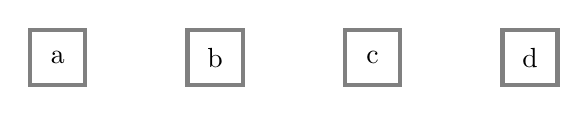
\begin{tikzpicture}[%
  node distance=2cm,
  nodestyle/.style={%
    rectangle,
    minimum width=2em,
    text centered,
    minimum height=2em,
    draw=black!50,
    ultra thick,
  }
]
  \node [nodestyle] (a) {a};
  \node [nodestyle, right of=a] (b) {b};
  \node [nodestyle, right of=b] (c) {c};
  \node [nodestyle, right of=c] (d) {d};
\end{tikzpicture}
\end{center}
with the following constraints:
\begin{align*}
& a \in \{1,2,3,4,5,6,7,8,9\} \\
& b \in \{0,1,2,3,4,5,6,7,8,9\} \\
& c \in \{0,1,2,3,4,5,6,7,8,9\} \\
& a \in \{1,3,5,7,9\} \\
\end{align*}

To randomly draw an odd number $abcd$ from $[1000,9999]$ is like drawing $a$ from $\{1,2,\ldots,9\}$, drawing $b,c$ from $\{0,1,\ldots,9\}$, with replacement, and drawing $d$ from $\{1,3,5,7,9\}$. Without the requirement of distinct digits, you could imagine drawing from the $4$ sets simultaneously. But the requirement of distinct digits puts a constraint on the drawing. You can no longer think of it as a simultaneous draw. But with some care, you can think of it as a sequential draw of the $4$ digits. Care is needed. If you first pick the last digit, $d$, then whichever digit you draw is no longer ``available'' when you go on to draw, say, the second digit $b$. On the other hand, if you draw $b$ first, it may or may not impact the probability of drawing $d$. That is, if you draw a $0$ for $b$, you still have $5$ choices for $d$, but if you draw a $1$ for $b$, you are left with only $4$ choices for $d$. Similarly, if you draw a $0$ for the third digit, $c$, say, it still leaves $9$ choices for the first digit $a$, whereas if you draw a $1$, it leaves only $8$ choices for $a$. Thus, to get the calculation right, you have to imagine a predetermined order of digit selection that ``works''. An order that works is $d,a,b,c$. Equivalently $d,a,c,b$. For the analogy with a sequential draw to work, you must draw $d$ first and $a$ second. So let's suppose you are drawing $d$ first ($5$ choices), that leaves one less digit for $a$ ($8$ choices), and subsequently one less digit for $b$ ($8$ choices), and lastly one less digit for $c$ ($7$ choices).

And thus, the probability is:
\begin{align*}
P & = \frac{5 \times 8 \times 8 \times 7}{9 \times 10 \times 10 \times 10} \\
  & = \frac{8 \times 7}{9 \times 5 \times 5} \\
  & = \frac{56}{225} \\
  & \simeq 24.9\%
\end{align*}

The correct answer is B. Our rough estimate of $25.2\%$, it turns out, was pretty accurate. 



\newpage
\section*{2. No Sport Days!}
\begin{question}
John plays soccer once every three days, plays basketball once every four days and plays volleyball every five days. He played all three sports on December 31st, 2018. How many days in 2019 did John not play any of the sports?

\begin{enumerate*}[label=\Alph*,itemjoin={\quad}]
  \item $78$
  \item $146$
  \item $144$
  \item $80$
  \item $152$
\end{enumerate*}
\end{question}

It helps to visualize the problem with a timeline. Figure~\ref{fig:sports:timeline} shows the first $60$ days. A brute-force strategy would be to extend the timeline to $365$ days and count the days where John played no sports. But it would be nicer to find another method. Note that on day $60$, all three sports are played. In a sense, everything ``resets'' on day $60$: day $61$ is like $1$st January. Since $6\times 60=360$, days $361$ and $362$ are no-sport days to be added to six times the count from $1$ to $60$. Looking at the figure, we count $24$ within the $60$-day period and so the answer is:
\begin{align*}
6 \times 24 + 2 = 146
\end{align*}
\begin{figure}[hptb]
\begin{minipage}[b]{\textwidth}
\centering
\includegraphics[width=\textwidth]%
{sports-timeline}
\caption{\textbf{The first $60$ days}.
\label{fig:sports:timeline}}
\end{minipage}
\end{figure}

If you can sketch a timeline fast enough, this could be a reasonable approach. Is there a more subtle approach? It is obvious that there will be no sports on prime-number days greater than $5$. It often helps to have memorized a bunch of prime numbers. Here you would need to quickly figure out this list:
\begin{align*}
&7, 11, 13, 17, 19, 23, 29, 31, 37, 41, 43, 47, 53, 59, 61, 67, 71, 73, 79, 83, 89, 97, 101, 103, 107, 109, 113, 127, 131, 137, \\&139, 149, 151, 157, 163, 167, 173, 179, 181, 191, 193, 197, 199, 211, 223, 227, 229, 233, 239, 241, 251, 257, 263, 269, \\&271, 277, 281, 283, 293, 307, 311, 313, 317, 331, 337, 347, 349, 353, 359
\end{align*}
But even that wouldn't be enough, because numbers of the form $2p$, for $p$ prime, are also no-sports day. For instance, $14$. So are numbers of the form $p_{a} \times p_{b}$, for $p_{a},p_{b}$ prime. For instance $7 \times 11=77$.

Another strategy is, instead, to count all sports days and deduct from $365$. That is more manageable. To calculate how many multiples of $3$ there are in $365$, divide the nearest, smaller multiple of $3$: $363/3=121$ are all soccer days. For soccer, basketball, volleyball, one gets:
\begin{align*}
\frac{363}{3} & = 121 \\
\frac{364}{4} & = 91 \\
\frac{365}{5} & = 73 \\
\end{align*}
However, multiples of $3 \times 4=12$ have been counted twice. And so have multiples of $3 \times 5$ and $4 \times 5$. 
\begin{align*}
\frac{360}{12} & = 30 \\
\frac{360}{15} & = 24 \\
\frac{360}{20} & = 18 \\
\end{align*}
If we add up the first three numbers and subtract the last three, we are getting closer, but there is still one problem. Consider $3 \times 4 \times 5=60$. $60$ is included among the $121$ multiples of $3$, among the $91$ multiples of $4$, and among the $73$ multiples of $5$. It is also among the $30$ multiples of $12$, among the $24$ multiples of $15$, and among the $18$ multiples of $20$. Thus by adding and subtracted we have in effect removed all the multiples of $60$. Since $360/60=6$, we must add those $6$ back in. In total,
\begin{align*}
121 + 91 + 73 - 30 - 24 - 18 + 6 & = 219 \\
365 - 219 & = 146
\end{align*}
The correct answer is B. 



\newpage
\section*{3. Congruent Circles and Angle}
\begin{question}
Two congruent circles centered at points $A$ and $B$ each pass through the other circle's center. The line containing both $A$ and $B$ is extended to intersect the circles at points $C$ and $D$. The circles intersect at two points, one of which is $E$. What is the degree measure of $\angle CED$?
\begin{enumerate*}[label=\Alph*,itemjoin={\quad}]
  \item $100\circ$
  \item $120\circ$
  \item $130\circ$
  \item $135\circ$
  \item $150\circ$
\end{enumerate*}
\end{question}

Refer to the figures on the next page. Triangle $AEB$ is equilateral, so $\angle AEB=60\circ$. Angle $\angle CAE$ is the complement of $\angle BAE$, so $\angle CAE=180-60=120\circ$. Triangle $CAE$ is isosceles, so $\angle CEA=30\circ$. Putting it together,
\begin{align*}
\angle CED 
  & = \angle CEA + \angle AEB + \angle BED \\
  & = 30\circ + 60\circ + 30\circ \\
  & = 120\circ
\end{align*}
The correct answer is B. 

\begin{figure}[hptb]
\begin{minipage}[b]{\textwidth}
\centering
\includegraphics[height=0.9\textheight]%
{congruent-circles}
%\caption{\textbf{Two Congruent Circles}.
%\label{fig:congruent-circles}}
\end{minipage}
\end{figure}



\newpage
\section*{4. Semi-Circle Inscribed in Triangle}
\begin{question}
A semicircle is inscribed in an isosceles triangle with base $16$ and height $15$ so that the diameter of the semicircle is contained in the base of the triangle as shown. What is the radius of the semicircle?
\begin{center}
\includegraphics[height=0.15\textheight]%
{semi-circle-triangle-1}
\end{center}
\begin{enumerate*}[label=\Alph*,itemjoin={\quad}]
  \item $4\sqrt{3}$
  \item $17\sqrt{2}$
  \item $17\sqrt{3}$
  \item $10$
  \item $\frac{120}{17}$
\end{enumerate*}
\end{question}

\begin{figure}[hptb]
\begin{minipage}[b]{\textwidth}
\centering
\includegraphics[height=0.3\textheight]%
{semi-circle-triangle-2}
\caption{\textbf{Semi-Circle Inscribed in a Triangle}.
\label{fig:semi:circle:triangle}}
\end{minipage}
\end{figure}


Refer to Figure~\ref{fig:semi:circle:triangle}. Triangles $ADB$ and $BDC$ are right-angled, i.e. $\angle ADB=90\circ$ and $\angle BDC=90\circ$. The known lengths are $AB=15$ and $BC=8$. Applying Pythagoras to $ABC$ yields:
\begin{align*}
AC = \sqrt{15^2 + 8^2} = \sqrt{289} = 17
\end{align*}
Applying Pythagoras to $ADB$ yields:
\begin{align*}
(17-x)^2 + r^2 = 15^2
\end{align*}
Applying Pythagoras to $BDC$ yields:
\begin{align*}
r^2 + x^2 = 8^2
\end{align*}
Subtracting the last two equations yields:
\begin{align*}
(17-x)^2 - x^2 & = 15^2 - 8^2 \\
17^2 - 2 \cdot 17 \cdot x + x^2 - x^2 & = 15^2 - 8^2 \\
x & = \frac{17^2 - 15^2 + 8^2}{2 \cdot 17} \\
\end{align*}
which we can use in $r^2=8^2-x^2$:
\begin{align*}
r^2 & = 8^2 - \left(\frac{17^2 - 15^2 + 8^2}{2 \cdot 17}\right)^2 \\
& = 64 - \left(\frac{289 - 225 + 64}{2 \cdot 17}\right)^2 \\
& = 64 - \left(\frac{64}{17}\right)^2 \\
& = \frac{64 \cdot 17^2 - 64^2}{17^2} \\
& = \frac{64(289-64)}{17^2} \\
& = \frac{64 \cdot 225}{17^2} \\
& = \frac{8^2 \cdot 15^2}{17^2} \\
\Rightarrow \hspace{2em}
r = \sqrt{r^2} & = \frac{8 \cdot 15}{17} \\
  & = \frac{120}{17}
\end{align*}
The correct answer is E. 

\end{document}